\documentclass[a4paper,10pt]{article}

\usepackage[utf8]{inputenc}
\usepackage[english]{babel}
%\usepackage[T1]{fontenc}
\usepackage{graphicx}
\usepackage{wrapfig}
\usepackage{amsmath, amssymb}
%\usepackage{listings}

\begin{document}

\author{Valentin Rosenberg, Zacharias Knudsen}
\date{\today}

\section{Linear regression}
The regression problem we are going to solve is predicting the amount of autothefts per population in communities. We did a 5-fold outer crossvalidation with an inner loop 10-fold crossvalidation and feature selection. 

\begin{figure}[ht]
   \centerline{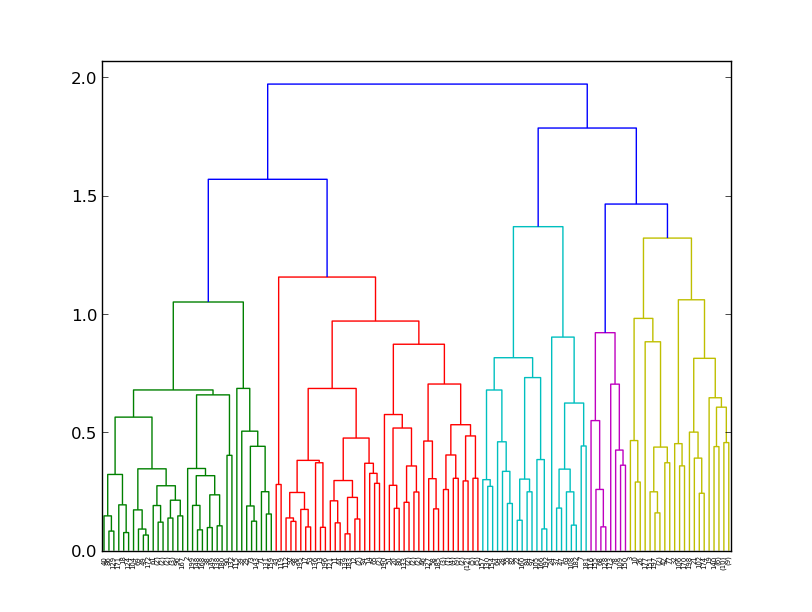
\includegraphics[width=1.3\textwidth]{figure_3.png}}
  \caption{Training of the model in third fold of crossvalidation}
\end{figure}

The fitting parameters show that our model benefits from feature selection, as both the error and fit of the model to the test are better with feature selection.
\begin{verbatim}
Linear regression without feature selection:

- Training error: 0.00522342840258
- Test error:     0.0631319627131
- R^2 train:     0.785850567012
- R^2 test:     -1.59138161533
Linear regression with feature selection:

- Training error: 0.00990016946312
- Test error:     0.0151810436296
- R^2 train:     0.594114150015
- R^2 test:     0.37686275426
\end{verbatim}

\subsection{}

\begin{figure}[ht]
   \centerline{\includegraphics[width=1.3\textwidth]{figure_10.png}}
  \caption{Predicted attribute with the true values and histogram of errors}
\end{figure}

\begin{figure}[ht]
   \centerline{\includegraphics[width=1.3\textwidth]{figure_61.png}}
  \caption{Residual error plots of some of the attributes}
\end{figure}

\subsection{}
The model coefficients of the linear model are shown below, in ordered list of the attributes and their coefficient value. policePerPop2 (unexplained in the dataset) and the number of persons living in urban areas are the most contributing attributes to the
\begin{verbatim}
['pctImmig-5' 'persPoverty' 'pctMaleDivorc' 'pctFemDivorc' 'persUrban'
 'policePerPop2']
[   1.88989563    2.27254948    2.88873715    3.5109234    97.79176162
  875.63649576]
\end{verbatim}

\begin{verbatim}
['policePerPop' 'pop' 'pctAllDivorc' 'policeField' 'pctImmig-8'
 'pctPersOwnOccup']
[-875.43290039  -98.96072598   -6.54728995   -2.31676831   -1.81957907
   -1.36791983]
\end{verbatim}

\subsection{}
We could not fit an Artificial neural network due to errors in our code we couldn't fix.

\subsection{}

\begin{verbatim}
Regressions are significantly different. (p=0.00179354397592)
\end{verbatim}


\begin{figure}[ht]
    \centerline{\includegraphics[width=1.3\textwidth]{figure_20.png}}
  \caption{lololol}
\end{figure}

\end{document}
